A \textit{regular icosahedron} is a $20$-faced solid where each face is an equilateral triangle and five triangles meet at every vertex. The regular icosahedron shown below has one vertex at the top, one vertex at the bottom, an upper pentagon of five vertices all adjacent to the top vertex and all in the same horizontal plane, and a lower pentagon of five vertices all adjacent to the bottom vertex and all in another horizontal plane. Find the number of paths from the top vertex to the bottom vertex such that each part of a path goes downward or horizontally along an edge of the icosahedron, and no vertex is repeated.\begin{center}
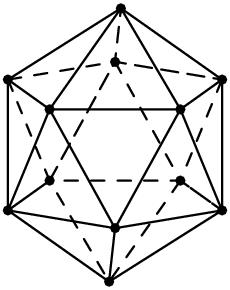
\includegraphics[width = 23.0mm]{img/fig0.png}
\end{center}